\chapter{数据表示、位级运算与浮点数}\label{CO02}

\par\medskip\noindent\textbf{章节脉络}\par\smallskip
\begin{wideblock}\centering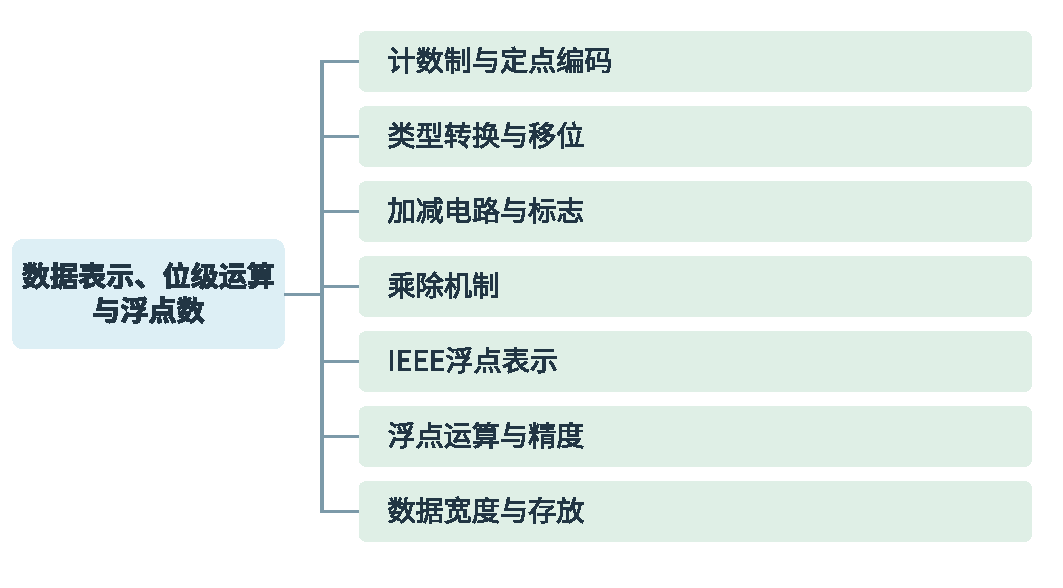
\includegraphics[width=\linewidth,height=92mm,keepaspectratio]{figures/overview.pdf}\end{wideblock}\par\medskip

本章围绕``计数制与定点编码 \ensuremath{\to} 类型转换与移位 \ensuremath{\to} 加减电路与标志 \ensuremath{\to} 乘除机制 \ensuremath{\to} IEEE浮点表示 \ensuremath{\to} 浮点运算与精度 \ensuremath{\to} 数据宽度与存放''展开。先判断对象与条件，再沿机制推导结果，最后用反例和数值检验结论。

\section{位串与数值之间还差一个解释规则}\label{CO02-02}

\begin{definition}[概念与适用对象]

位是取0或1的二进制位，字节 B 在本讲义中为8位，bit 写作 b。同一位串可以解释成无符号整数、补码整数、浮点数或字符编码。计算前必须同时确定\textbf{位宽、编码和小数点位置}，不能看见最高位为1就断言``这个数是负数''。

\end{definition}

\(r\) 进制采用位置权，\((a_k\cdots a_0.a_{-1}\cdots)_r\) 的值是 \(\sum_i a_i r^i\)，其中 \(0\le a_i<r\)。二进制与八进制、十六进制转换时，从小数点向两侧分组：每3位一组对应一位八进制，每4位一组对应一位十六进制；整数端左侧补0，小数端右侧补0。

\subsection{例 2-1　整数与小数分别换基数}\label{CO02-03}

\begin{example}[配套例题]

【配套例题】 若十进制数为137.5，则其八进制数为（　）。

A. 89.8　 B. 211.4　 C. 211.5　 D. 1011111.101

\end{example}

\textbf{解析。} \(137=2\times8^2+1\times8+1\)，小数部分 \(0.5\times8=4\)，因此为 \((211.4)_8\)，选 \textbf{B}。八进制数字只能是0至7，A 本身就不是合法八进制数。分组也可验证：\(137.5=(10001001.1)_2=(010\ 001\ 001.100)_2\)。

十进制整数转二进制可反复除2取余、倒序排列；小数则反复乘2取整数、顺序排列。有限十进制小数未必能写成有限二进制小数，例如0.1的二进制表示无限循环。保存有限位时会发生近似，这正是后面浮点舍入出现的原因之一。

\section{定点编码：范围先于运算规则}\label{CO02-04}

真值是按通常数学符号写出的数值；机器数是采用约定编码保存的位串。定点表示约定小数点位置固定，并不表示存储器真的另存了一个小数点。

对 \(n\) 位整数，常用编码如下。

\begin{wideblock}

\par\medskip\noindent\begin{minipage}{\linewidth}\fontsize{9.3}{12}\selectfont\begin{tabularx}{\linewidth}{@{}YYY@{}}
\toprule\noalign{}
\begin{minipage}[b]{\linewidth}\raggedright
编码
\end{minipage} & \begin{minipage}[b]{\linewidth}\raggedright
最高位和数值含义
\end{minipage} & \begin{minipage}[b]{\linewidth}\raggedright
表示范围
\end{minipage} \\
\midrule\noalign{}


无符号 & 所有位均有正权 & \(0\) 至 \(2^n-1\) \\
原码 & 最高位为符号，其余为绝对值 & \(-(2^{n-1}-1)\) 至 \(2^{n-1}-1\)，两个零 \\
反码 & 正数同原码，负数的数值位取反 & 与原码相同，两个零 \\
补码 & 最高位权为 \(-2^{n-1}\)，其余为正权 & \(-2^{n-1}\) 至 \(2^{n-1}-1\)，一个零 \\
\bottomrule\end{tabularx}
\end{minipage}\par\medskip

\end{wideblock}

8位补码 \texttt{1111 1101} 的值为 \(-128+64+32+16+8+4+1=-3\)。也可先把它作为无符号数253，再因最高位为1减去256，得到\ensuremath{-}3。后一方法适合十六进制机器数：对 \(n\) 位补码，若无符号解释为 \(u\)，则最高位为 0 时取 \(u\)，为 1 时取 \(u-2^n\)。

求一个负整数的补码时，可在给定位宽下把它的绝对值逐位取反再加1；位宽不能省。8位中 \(-128\) 编码为 \texttt{1000 0000}，它的数学相反数128不能用8位补码表示。``取反加1''得到的仍是同一位串，这说明运算按模256进行，并不表示已经得到可表示的正128。

原码中的 \texttt{1000 0000} 表示\ensuremath{-}0，补码中则表示\ensuremath{-}128。反码的\ensuremath{-}0是 \texttt{1111 1111}。对于常见的偏置 \(2^{n-1}\) 的整数移码，有 \(E=x+2^{n-1}\)，与对应补码相比只需翻转最高位；IEEE 754 阶码的偏置通常为 \(2^{k-1}-1\)，不可套用``翻转最高位''这一特殊关系。

若采用一位符号、\(n-1\) 位小数的补码定点小数，最高位权为\ensuremath{-}1，其余权从 \(2^{-1}\) 至 \(2^{-(n-1)}\)，范围为 \([-1,1-2^{-(n-1)}]\)。同样的位串改变小数点位置，真值就按2的幂缩放。

\section{截断、扩展与 C 类型转换}\label{CO02-05}

位宽变小时，硬件截取低位；能否保留原数值，要检查被丢掉的位。位宽增大时，无符号数在高位补0，有符号补码数复制符号位。原码、反码各有自己的扩展规则，补码规则并不适用于所有编码。

8位补码\ensuremath{-}3扩为16位是 \texttt{1111 1111 1111 1101}，无符号253扩为16位则是 \texttt{0000 0000 1111 1101}。扩展后低8位相同，真值不同。\textbf{扩展方式首先取决于源数怎样解释，而不是目标类型名字中有没有 unsigned。}

\subsection{例 2-2　无符号短整数扩展}\label{CO02-06}

\begin{example}[配套例题]

【配套例题】 假定编译器规定 int 型和 short 型长度分别为32位和16位，执行下列 C 语言语句：

\par\medskip\noindent\begin{minipage}{\linewidth}
\begin{codeblock}[language=C]
unsigned short x = 65530;
unsigned int y = x;
\end{codeblock}
\end{minipage}\par\medskip

得到 y 的机器数为（　）。

A. 0000 7FFAH　 B. 0000 FFFAH　 C. FFFF 7FFAH　 D. FFFF FFFAH

\end{example}

\textbf{解析。} \(65530=65536-6=\mathtt{FFFAH}\)，源类型是无符号16位数，扩展补0，得到 \texttt{0000 FFFAH}，选 \textbf{B}。最高位为1在这里是普通数值位，不是负号。

\subsection{例 2-3　负的 short 转成 unsigned int}\label{CO02-07}

\begin{example}[配套例题]

【配套例题】 在32位计算机上执行下列 C 语言代码段后，ui 的值是（　）。

\par\medskip\noindent\begin{minipage}{\linewidth}
\begin{codeblock}[language=C]
short si = -32767;
unsigned int ui = si;
\end{codeblock}
\end{minipage}\par\medskip

A. \(2^{15}-1\)　 B. \(2^{15}+1\)　 C. \(2^{32}-2^{15}-1\)　 D. \(2^{32}-2^{15}+1\)

\end{example}

\textbf{解析。} 按题目的16位 short、32位 unsigned int 模型，\ensuremath{-}32767的16位补码为 \texttt{8001H}。数值转换为32位无符号整数后，得到与\ensuremath{-}32767模 \(2^{32}\) 同余的数，即 \(2^{32}-32767=2^{32}-2^{15}+1\)，机器数为 \texttt{FFFF 8001H}，选 \textbf{D}。把 \texttt{8001H} 直接补0会把负的源值误当成无符号32769。

C 中的 usual arithmetic conversions 也会改变比较方式。若32位 \texttt{int i=\allowbreak{}-1} 与32位 \texttt{unsigned u=\allowbreak{}1} 比较，常见模型下 i 转为无符号 \(2^{32}-1\)，所以 \texttt{i<\allowbreak{}u} 为假。需要先完成整数提升和通常算术转换，再决定按哪种值比较。

本讲义中``截断取低位''的位级推演按题设机器模型进行。C 语言本身不保证有符号溢出按补码绕回：有符号加法溢出属于未定义行为；按本讲义采用的 C11/C17 口径，超范围转换到有符号类型还涉及实现规定。考题若明确给机器位宽和截断模型，可据模型计算；编写可移植 C 程序时不能把这些题设当成语言的普遍保证。

\subsection{移位先问逻辑还是算术}\label{CO02-08}

逻辑右移高位补0，算术右移复制符号位；左移均在低位补0，但如何解释结果及是否溢出仍取决于编码。8位补码\ensuremath{-}3算术右移1位得到\ensuremath{-}2，相当于向负无穷方向取整；整数除法\ensuremath{-}3/2通常向零截断得到\ensuremath{-}1，两者不能无条件互换。左移时被丢弃的高位无法恢复，``低位补0''也不保证数值恰好乘2。

\section{加法器怎样同时支持加与减}\label{CO02-09}

一位全加器接收 \(A_i,B_i,C_i\)，产生和位 \(S_i\) 与向高位的进位 \(C_{i+1}\)：

\[
S_i=A_i\oplus B_i\oplus C_i,
\qquad C_{i+1}=A_iB_i+(A_i\oplus B_i)C_i.
\]

定义进位生成 \(G_i=A_iB_i\)、进位传递 \(P_i=A_i\oplus B_i\)，即可逐层展开进位表达式。串行进位需等低位进位逐级传播；先行进位用更复杂的组合逻辑并行形成若干进位，缩短关键路径。更快的进位结构没有改变加法的数值规则。

加减运算器用控制位 Sub 将第二输入按位与 Sub 异或，同时令最低进位 \(C_0=\mathrm{Sub}\)。Sub=0时执行 \(A+B\)；Sub=1时执行 \(A+\overline B+1\)，即模 \(2^n\) 的减法。算术逻辑部件 ALU 还通过选择控制实现与、或、异或等逻辑操作；移位器是否算在 ALU 内部，要看具体的数据通路图。

\subsection{例 2-4　减法器的两路输入不直接送负数符号}\label{CO02-10}

\begin{example}[配套例题]

【配套例题】 某计算机字长为8位，CPU 中有一个8位加法器。已知无符号数 \(x=69,y=38\)，若在该加法器中计算 \(x-y\)，则加法器的两个输入端信息和输入的低位进位信息分别为（　）。

A. 0100 0101、0010 0110、0\\
B. 0100 0101、1101 1001、1\\
C. 0100 0101、1101 1010、0\\
D. 0100 0101、1101 1010、1

\end{example}

\textbf{解析。} \(69=0100\ 0101\)，\(38=0010\ 0110\)。第二路取反为 \texttt{1101 1001}，另由最低进位补上1，所以选 \textbf{B}。若第二路已取反加1又令最低进位为1，就重复加了1。运算实际为 \(69+217+1=287\)，低8位31、最高进位1，符合 \(69-38=31\)。

\section{CF 与 OF 分别判断什么}\label{CO02-11}

同一次加法器运算可以同时按有符号和无符号两种规则解释，因此产生不同用途的标志。ZF 表示结果低 \(n\) 位是否全0，SF 等于结果最高位；SF=1并不自动表示数学真值为负，还要确认按有符号解释且未发生有符号溢出。

对于加法，CF 反映最高位向外进位；对于本讲义采用的``CF=1表示借位''约定，减法的 CF 为最高进位的反值。可统一写为 \(\mathrm{CF}=C_n\oplus\mathrm{Sub}\)。某些 ISA 用``无借位''作为减法进位标志，遇到这类题设时，必须按该 ISA 的约定判断。

OF 判断有符号结果是否越出补码范围：加法时同号相加而结果异号会溢出；减法时两操作数异号且结果符号与被减数不同会溢出。也可用符号位的进位输入与进位输出异或：\(\mathrm{OF}=C_{n-1}\oplus C_n\)。它不要求把符号位当成独立的符号去做原码运算。

\subsection{同一个结果，按哪一种数判断}\label{CO02-12}

位串运算、数值解释和条件判断应分三步。先按位宽完成加减，保留低 \(n\) 位；再按无符号或补码规则解读；最后选择与这种解释对应的标志。不能为了得到希望的正负号，改写已经产生的机器结果。

\begin{wideblock}\par\medskip\noindent\begin{minipage}{\linewidth}\fontsize{9.3}{12}\selectfont\begin{tabularx}{\linewidth}{@{}YYYY@{}}
\toprule\noalign{}
8位运算 & 保留结果 & 按无符号解释 & 按补码解释 \\
\midrule\noalign{}


\texttt{7FH+\allowbreak{}01H} & \texttt{80H} & \(127+1=128\)，可表示 & \(127+1\) 超过127 \\
\texttt{FFH+\allowbreak{}01H} & \texttt{00H} & \(255+1\) 超过255 & \(-1+1=0\)，可表示 \\
\texttt{80H-01H} & \texttt{7FH} & \(128-1=127\)，无借位 & \(-128-1\) 小于\ensuremath{-}128 \\
\texttt{00H-01H} & \texttt{FFH} & \(0-1\) 需借位 & \(0-1=-1\)，可表示 \\
\bottomrule\end{tabularx}
\end{minipage}\par\medskip\end{wideblock}

同一过程的其余状态（按首列对应）：

\par\medskip\noindent\begin{minipage}{\linewidth}\fontsize{9.3}{12}\selectfont\begin{tabularx}{\linewidth}{@{}YY@{}}
\toprule\noalign{}
8位运算 & CF、OF \\
\midrule\noalign{}


\texttt{7FH+\allowbreak{}01H} & 0、1 \\
\texttt{FFH+\allowbreak{}01H} & 1、0 \\
\texttt{80H-01H} & 0、1 \\
\texttt{00H-01H} & 1、0 \\
\bottomrule\end{tabularx}
\end{minipage}\par\medskip

ZF和SF只看保留下来的结果：上表第二行ZF=1，第一行与第四行SF=1。若要由减法结果判断补码数的有符号小于或大于关系，应结合OF修正结果符号；例如第三行SF=0，却不能据此说原来的\ensuremath{-}128大于1。是否相等只需看ZF，不必额外使用OF。编码范围决定“能否表示”，运算电路决定“产生哪些位”，转移条件决定“怎样使用标志”，三者要连起来判断。

\subsection{例 2-5　十六进制补码相减}\label{CO02-13}

\begin{example}[配套例题]

【配套例题】 假定有符号整数采用补码表示，若 int 型变量 x 和 y 的机器数分别是 FFFF FFDFH 和0000 0041H，则 x、y 的值及 x\ensuremath{-}y 的机器数分别是（　）。

A. x=\ensuremath{-}65，y=41，x\ensuremath{-}y 的机器数溢出\\
B. x=\ensuremath{-}33，y=65，x\ensuremath{-}y 的机器数为 FFFF FF9DH\\
C. x=\ensuremath{-}33，y=65，x\ensuremath{-}y 的机器数为 FFFF FF9EH\\
D. x=\ensuremath{-}65，y=41，x\ensuremath{-}y 的机器数为 FFFF FF96H

\end{example}

\textbf{解析。} \texttt{FFFFFFDFH} 距 \(2^{32}\) 差33，故 x=\ensuremath{-}33；\texttt{41H} 是十进制65。数学结果为\ensuremath{-}98，在32位补码范围内，机器数为 \(2^{32}-98=\mathtt{FFFFFF9EH}\)，选 \textbf{C}。十六进制的41不能按十进制41读。

\subsection{例 2-6　有符号减法为何仍会产生借位}\label{CO02-14}

\begin{example}[配套例题]

【配套例题】 已知 x、y 为 int 类型，当 x=100、y=200时，执行``x减y''指令得到的溢出标志 OF 和借位标志 CF 分别为0、1。那么当 x=10、y=\ensuremath{-}20时，执行该指令得到的 OF 和 CF 分别是（　）。

A. OF=0，CF=0　 B. OF=0，CF=1　 C. OF=1，CF=0　 D. OF=1，CF=1

\end{example}

\textbf{解析。} 有符号真值为 \(10-(-20)=30\)，可表示，OF=0。若按无符号解释输入位串，\ensuremath{-}20对应 \(2^{32}-20\)，10小于它，减法需要借位，CF=1，选 \textbf{B}。题目已经用100\ensuremath{-}200说明了借位标志约定，不能把两个标志都按有符号真值判断。

条件转移利用这些标志完成比较。先计算 \(a-b\)：无符号 \(a<b\) 对应 CF=1，无符号 \(a>b\) 对应 CF=0且ZF=0；带符号 \(a<b\) 对应 \(\mathrm{SF}\ne\mathrm{OF}\)，带符号 \(a>b\) 对应ZF=0且SF=OF。用 SF 单独判断带符号大小，会在溢出时失败。

\section{乘除运算必须保留的中间量}\label{CO02-15}

\subsection{无符号乘法：为什么需要部分积和双倍位宽}\label{CO02-16}

两个 \(n\) 位无符号数的精确乘积最多需要 \(2n\) 位。以王道书§2.2中的13乘11为例：\(13=1101_2\)，\(11=1011_2\)。乘数从低位到高位为1、1、0、1，部分积依次是13、26、0、104，总和143，即 \texttt{1000 1111}。

顺序乘法器可以每轮检查乘数最低位，决定是否把被乘数加到部分积高半部，再将``进位---部分积---乘数''组合右移。部分积开始为0，循环 \(n\) 次后得到 \(2n\) 位积。相应的等价算法也可让被乘数左移、乘数右移，把选中的部分积加到双倍宽累加器；两种寄存器布局的逐轮数值不同，不应把一种布局的移位规则套用到另一种。

对13\ensuremath{\times}11，用双倍宽累加器的轨迹如下：

\begin{wideblock}\par\medskip\noindent\begin{minipage}{\linewidth}\fontsize{9.3}{12}\selectfont\begin{tabularx}{\linewidth}{@{}YYYY@{}}
\toprule\noalign{}
本轮乘数低位 & 本轮被乘数 & 累加器更新后 & 乘数右移后 \\
\midrule\noalign{}


1 & 13 & 13 & 5 \\
1 & 26 & 39 & 2 \\
0 & 52 & 39 & 1 \\
1 & 104 & 143 & 0 \\
\bottomrule\end{tabularx}
\end{minipage}\par\medskip\end{wideblock}

带符号乘法不能把负数的补码直接当成同宽无符号数求完整积。Booth 法在乘数末端附一位0，考察相邻两位 \(q_iq_{i-1}\)：01时加被乘数，10时减被乘数，00或11不加减，再对组合寄存器算术右移。这里的前提是符号扩展到位、中间寄存器足够宽；对最小负数取负时，尤其需要保护位。

以4位补码的\ensuremath{-}3\ensuremath{\times}5说明Booth法（原创机制示例）。乘数寄存器Q为4位，附加位\(q_{-1}\)为1位，A采用5位补码以保留保护位，被乘数M=\ensuremath{-}3也扩成5位。初态A=\texttt{00000}、Q=\texttt{0101}、\(q_{-1}=0\)。每轮先看\(Q_0q_{-1}\)，对A加减M，再把A、Q、\(q_{-1}\)连接成10位整体算术右移；A的最低位移入Q最高位，Q最低位移入\(q_{-1}\)。

\begin{wideblock}\par\medskip\noindent\begin{minipage}{\linewidth}\fontsize{9.3}{12}\selectfont\begin{tabularx}{\linewidth}{@{}YYYY@{}}
\toprule\noalign{}
轮次 & 判断位 & 移位前操作及A真值 & 移位后的A \\
\midrule\noalign{}


1 & 10 & A\ensuremath{-}M=3 & 00001 \\
2 & 01 & A+M=\ensuremath{-}2 & 11111 \\
3 & 10 & A\ensuremath{-}M=2 & 00001 \\
4 & 01 & A+M=\ensuremath{-}2 & 11111 \\
\bottomrule\end{tabularx}
\end{minipage}\par\medskip\end{wideblock}

同一过程的其余状态（按首列对应）：

\par\medskip\noindent\begin{minipage}{\linewidth}\fontsize{9.3}{12}\selectfont\begin{tabularx}{\linewidth}{@{}YYY@{}}
\toprule\noalign{}
轮次 & 移位后的Q & \(q_{-1}\) \\
\midrule\noalign{}


1 & 1010 & 1 \\
2 & 0101 & 0 \\
3 & 0010 & 1 \\
4 & 0001 & 0 \\
\bottomrule\end{tabularx}
\end{minipage}\par\medskip

四轮后AQ为9位\texttt{11111 0001}，去掉冗余符号保护位即8位\texttt{1111 0001}，真值为\ensuremath{-}15。移位时必须复制A的符号位，并在寄存器边界传位；把A、Q分别右移会丢掉跨界位，得到错误乘积。

阵列乘法器用组合电路完成部分积生成与压缩求和，可能在一个足够长的时钟周期内完成；顺序乘法器复用 ALU 和移位器，通常跨多个周期。``一个周期''不能脱离所用电路和时钟周期长度讨论。常数乘法可以在保持规定语义的前提下化为移位与加减，例如 \(13x=(x\ll3)+(x\ll2)+x\)。

\subsection{除法：商来自每一步余数比较}\label{CO02-17}

以无符号7÷3为例，按被除数的有效位 \texttt{111} 从高到低处理，初始余数 R=0。每读入一位，先令 \(R\leftarrow2R+b\)，若 R\ensuremath{\ge}3则减3并在商中记1，否则记0。

\begin{wideblock}\par\medskip\noindent\begin{minipage}{\linewidth}\fontsize{9.3}{12}\selectfont\begin{tabularx}{\linewidth}{@{}YYYY@{}}
\toprule\noalign{}
读入位 & 比较前余数 & 本位商 & 本步余数 \\
\midrule\noalign{}


1 & 1 & 0 & 1 \\
1 & 3 & 1 & 0 \\
1 & 1 & 0 & 1 \\
\bottomrule\end{tabularx}
\end{minipage}\par\medskip\end{wideblock}

商为 \texttt{010} 即2，余数1，满足 \(7=2\times3+1\) 且 \(0\le R<3\)。硬件通常固定处理整个位宽，在前面补零位，不会因此改变结果。恢复余数法先试减，结果为负时再加回除数；不恢复余数法根据余数符号决定下一轮加还是减，用不同轨迹完成同一任务。

不恢复余数法也可用同一7÷3观察。令余数R为4位有符号寄存器、Q为3位，除数D=3，初态R=0、Q=\texttt{111}。每轮先把R、Q连接左移一位，Q最高位移入R最低位；若上一轮R非负，本轮减D，若上一轮R为负则加D；运算后R非负就在Q最低位置1，否则置0。

\begin{wideblock}\par\medskip\noindent\begin{minipage}{\linewidth}\fontsize{9.3}{12}\selectfont\begin{tabularx}{\linewidth}{@{}YYYY@{}}
\toprule\noalign{}
轮次 & 左移后R真值 & 加减操作 & 操作后R \\
\midrule\noalign{}


1 & 1 & R\ensuremath{-}D & \ensuremath{-}2 \\
2 & \ensuremath{-}3 & R+D & 0 \\
3 & 1 & R\ensuremath{-}D & \ensuremath{-}2 \\
\bottomrule\end{tabularx}
\end{minipage}\par\medskip\end{wideblock}

同一过程的其余状态（按首列对应）：

\par\medskip\noindent\begin{minipage}{\linewidth}\fontsize{9.3}{12}\selectfont\begin{tabularx}{\linewidth}{@{}YY@{}}
\toprule\noalign{}
轮次 & 记商后的Q \\
\midrule\noalign{}


1 & 110 \\
2 & 101 \\
3 & 010 \\
\bottomrule\end{tabularx}
\end{minipage}\par\medskip

最后R仍负，补做R\ensuremath{\leftarrow}R+D，得到余数1，Q=\texttt{010}为商2。第二轮没有先把\ensuremath{-}2恢复成1再试减，而把恢复效果合并进下一轮加法，这正是不恢复余数法的含义；最终余数校正不能漏掉。硬件布局或商编码约定不同会改变表中轨迹，做题时应遵循同一套规则。

有符号除法还要确定商、余数符号和舍入方向。按 C 向零截断模型，\ensuremath{-}7÷3的商为\ensuremath{-}2、余数为\ensuremath{-}1，仍满足被除数=商\ensuremath{\times}除数+余数。除数为0时需要异常处理；\(-2^{n-1}/(-1)\) 的商超出 \(n\) 位补码范围。某种除法器可能检测到被除数绝对值小于除数，就提前输出商0；另一种固定轮数除法器仍运行完整迭代。只有题干电路给出提前退出逻辑时，才能比较哪组数据用时最短。

\section{IEEE 754：字段既规定精度，也规定特殊情况}\label{CO02-18}

IEEE 754 binary32 即通常的单精度格式，由1位符号 s、8位阶码 E、23位尾数字段 F 构成；binary64分别为1、11、52位。这里 F 的整数值要除以 \(2^{23}\) 或 \(2^{52}\) 才是小数尾数部分。

\par\medskip\noindent\begin{minipage}{\linewidth}\fontsize{9.3}{12}\selectfont\begin{tabularx}{\linewidth}{@{}YYY@{}}
\toprule\noalign{}
项目 & binary32（单精度） & binary64（双精度） \\
\midrule\noalign{}


总位数 & 32位 & 64位 \\
符号位 \(s\) & 1位 & 1位 \\
阶码 \(E\) & 8位 & 11位 \\
尾数字段 \(F\) & 23位 & 52位 \\
阶码偏置 \(B\) & 127 & 1023 \\
规格化数的真阶码 \(e\) & \(-126\le e\le127\) & \(-1022\le e\le1023\) \\
规格化数的有效精度 & 24位，含隐含前导1 & 53位，含隐含前导1 \\
\bottomrule\end{tabularx}
\end{minipage}\par\medskip

\par\medskip\noindent\begin{minipage}{\linewidth}\fontsize{9.3}{12}\selectfont\begin{tabularx}{\linewidth}{@{}YYY@{}}
\toprule\noalign{}
项目 & binary32（单精度） & binary64（双精度） \\
\midrule\noalign{}


最小正规格化数 & \(2^{-126}\) & \(2^{-1022}\) \\
最小正非规格化数 & \(2^{-149}\) & \(2^{-1074}\) \\
最大有限正数 & \((2-2^{-23})2^{127}\) & \((2-2^{-52})2^{1023}\) \\
\bottomrule\end{tabularx}
\end{minipage}\par\medskip

\par\medskip\noindent\begin{minipage}{\linewidth}
\centering
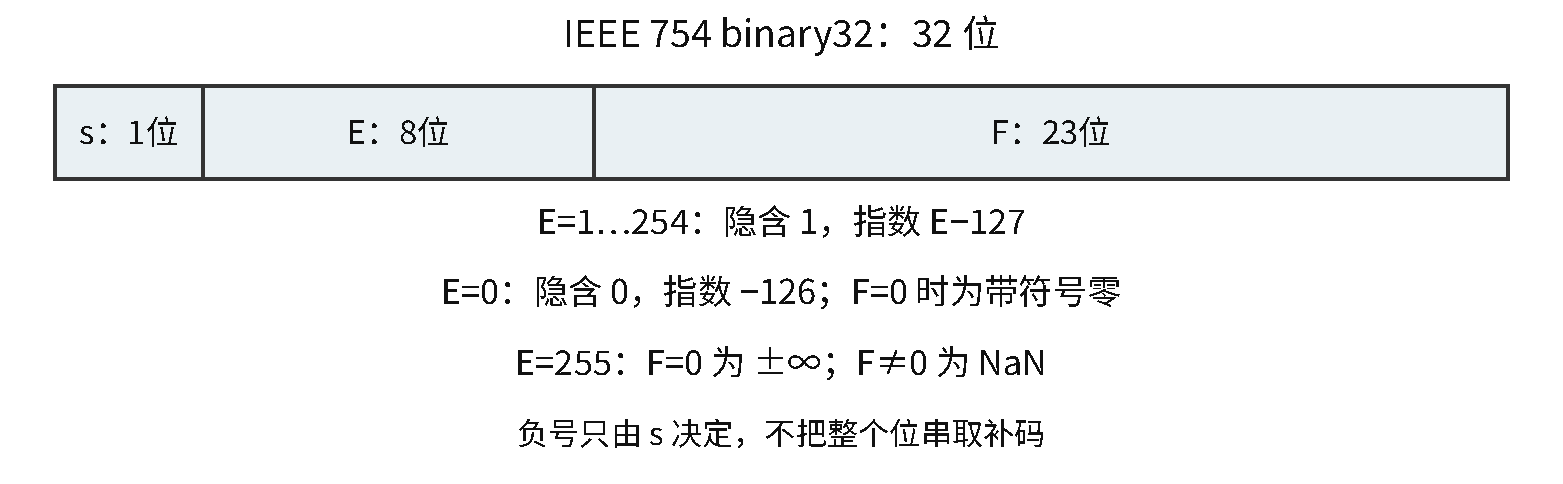
\includegraphics[width=\linewidth,height=125mm,keepaspectratio]{figures/CO_F01_ieee754.pdf}
\captionof{figure}{单精度字段及三类指数编码}
\end{minipage}\par\medskip

解码时先看阶码是否全0或全1，再看尾数字段。下表中 \(p\) 是尾数字段位数，binary32取23、binary64取52；\(B\) 是对应的阶码偏置，\(F\) 按无符号整数解释。

\begin{wideblock}\par\medskip\noindent\begin{minipage}{\linewidth}\fontsize{9.3}{12}\selectfont\begin{tabularx}{\linewidth}{@{}YYYY@{}}
\toprule\noalign{}
\begin{minipage}[b]{\linewidth}\raggedright
类别
\end{minipage} & \begin{minipage}[b]{\linewidth}\raggedright
阶码 \(E\)
\end{minipage} & \begin{minipage}[b]{\linewidth}\raggedright
尾数字段 \(F\)
\end{minipage} & \begin{minipage}[b]{\linewidth}\raggedright
数值或含义
\end{minipage} \\
\midrule\noalign{}


正零、负零 & 全0 & 0 & \((-1)^s0\)，符号位区分正负零 \\
非规格化数 & 全0 & 非0 & \((-1)^s(F/2^p)2^{1-B}\)，隐含前导0 \\
规格化数 & 既非全0，也非全1 & 任意 & \((-1)^s(1+F/2^p)2^{E-B}\)，隐含前导1 \\
正无穷、负无穷 & 全1 & 0 & \((-1)^s\infty\) \\
NaN & 全1 & 非0 & 非数；不能当作无穷或普通实数 \\
\bottomrule\end{tabularx}
\end{minipage}\par\medskip\end{wideblock}

对于 binary32：

\[
x=\begin{cases}
(-1)^s(1+F/2^{23})2^{E-127},&1\le E\le254;\\
(-1)^s(F/2^{23})2^{-126},&E=0;\\
(-1)^s\infty,&E=255,F=0;\\
\mathrm{NaN},&E=255,F\ne0.
\end{cases}
\]

规格化数有隐含的前导1，有效精度24位。非规格化数前导为0，最小指数同样取\ensuremath{-}126，数值逐渐接近0；当 F=0时是带符号零。非规格化数不能再用指数 E\ensuremath{-}127配隐含1计算。

最小正规格化数为 \(2^{-126}\)，最小正非规格化数为 \(2^{-149}\)，最大有限正数为 \((2-2^{-23})2^{127}\)。这些是数值范围；``能连续精确表示的整数''是另一问题。binary32能精确表示 \([-2^{24},2^{24}]\) 内所有整数，更大的某些整数仍能精确表示，但相邻可表示数的间隔可能大于1。

\subsection{例 2-7　负小数怎样组成单精度机器数}\label{CO02-19}

\begin{example}[配套例题]

【配套例题】 \ensuremath{-}0.4375的 IEEE 754 单精度浮点数表示为（　）。

A. BEE0 0000H　 B. BF60 0000H　 C. BF70 0000H　 D. C0E0 0000H

\end{example}

\textbf{解析。} \(0.4375=0.0111_2=1.11_2\times2^{-2}\)。

s=1，E=\ensuremath{-}2+127=125=\texttt{01111101}，F为 \texttt{110} 后补20个0。

连接为 \texttt{1|01111101|11000000000000000000000}，十六进制为 \texttt{BEE00000H}，选 \textbf{A}。负数只改变符号位，不对浮点数全部位取补码。

\subsection{例 2-8　同为负浮点数时怎样比较}\label{CO02-20}

\begin{example}[配套例题]

【配套例题】 float 型数据常用 IEEE 754 单精度浮点格式表示。假设两个 float 型变量 x 和 y 分别存放在32位寄存器 f1 和 f2 中，若 \texttt{(\allowbreak{}f1)\allowbreak{}=\allowbreak{}CC90 0000H}、\texttt{(\allowbreak{}f2)\allowbreak{}=\allowbreak{}B0C0 0000H}，则 x 和 y 之间的关系为（　）。

A. x\textless y且符号相同　 B. x\textless y且符号不同　 C. x\textgreater y且符号相同　 D. x\textgreater y且符号不同

\end{example}

\textbf{解析。} 两个最高位都为1，均为负。x的阶码为153，实际指数26；y的阶码为97，实际指数\ensuremath{-}30。两者均为有限规格化数，x的绝对值远大于y，因此 x\textless y，选 \textbf{A}。此处不必把尾数展开为完整十进制数。对负数，绝对值更大的反而更小。

int 转 float 可能丢低位，32位 int 转 binary64 则可精确表示，因为 binary64 有53位有效精度。float 转 double 在通常 IEEE 格式下能精确保留原来的有限数值，但不能恢复 float 形成时已经丢掉的信息。浮点转整数按语言规则截断，且须检查范围；NaN 与任何数（包括自身）的相等比较都为假，不能把 \texttt{x/\allowbreak{}x=\allowbreak{}=\allowbreak{}1} 用在 x=0或无穷等情形。

\section{浮点加减：对阶丢位以后还要判断舍入}\label{CO02-21}

两个浮点数只有指数相同，才能直接把有效数相加。通常先把较小指数的有效数右移，使指数与较大者一致；这叫对阶。大阶向小阶对齐会要求更多高位和更大的寄存器，不符合固定精度运算的通常实现。

对阶之后进行尾数运算，再规格化和舍入。加法可能得到 \(10.xxx_2\)，须右移1位、阶码加1；异号相加发生抵消，可能得到 \(0.00\cdots1xxx_2\)，须左移、阶码减少。舍入使尾数加1时还可能再次进位，必须再检查规格化和阶码范围。若得到精确的0，也不能继续无止境地左移寻找前导1。

用一个仅保留4位有效数的教学格式说明舍入。\(x=1.000_2\times2^0\)，\(y=1.000_2\times2^{-4}\)，精确和为 \(1.0001_2\)，恰好位于保留为 \texttt{1.\allowbreak{}000} 和 \texttt{1.\allowbreak{}001} 的中点。采用``舍入到最近，正中取偶数''，保留最低位为0的 \texttt{1.\allowbreak{}000}。若 x 改为 \texttt{1.\allowbreak{}001}，精确和为 \texttt{1.\allowbreak{}0011}，则正中取偶数进为 \texttt{1.\allowbreak{}010}。偶数指保留有效数的最低位为0，不是判断整个真值是奇整数还是偶整数。

实际实现常保留保护位、舍入位和粘滞位。粘滞位记录更低位中是否出现过1，因此 \texttt{1000…} 与 \texttt{1000…1} 的舍入结论可能不同，不能只保留移出的第一位。

\subsection{例 2-9　哪些步骤可能造成指数越界}\label{CO02-22}

\begin{example}[配套例题]

【配套例题】 下列有关浮点数加减运算的叙述中，正确的是（　）。

I. 对阶操作不会引起阶码上溢或下溢\\
II. 右规和尾数舍入都可能引起阶码上溢\\
III. 左规时可能引起阶码下溢\\
IV. 尾数溢出时，结果不一定溢出

A. 仅 II、III　 B. 仅 I、II、IV　 C. 仅 I、III、IV　 D. I、II、III、IV

\end{example}

\textbf{解析。} 对阶把较小阶提高到较大阶，最终阶码仍是原有合法阶码之一；右移尾数可能损失精度，但不使该阶码越界，I正确。右规和舍入后的再右规会使指数加1，可能越过上界，II正确。抵消后的左规要减小指数，可能进入非规格化区或触及题设的下溢界，III正确。尾数暂时形成 \texttt{10.\allowbreak{}xxx} 还可以右规，只要指数容纳得下，结果仍可表示，IV正确。选 \textbf{D}。尾数的暂时进位与最终浮点范围溢出是不同层次。

采用 IEEE 754 的渐进下溢时，指数过小并不立即把所有结果变成0，还可能形成非规格化数。题目若采用``阶码、尾数均为补码''的教学格式，就应按其位宽、小数点位置、双符号位和舍入方法计算，不能把该格式的尾数补码接到 IEEE 字段中。

浮点加法不满足数学实数的结合律。例如在 binary32 中，\(a=2^{25},b=-2^{25},c=1\)：\((a+b)+c=1\)，而 \(a+(b+c)\) 中 b+c 可能先舍入回 b，结果为0。发生差异的原因是中间舍入，不是加法指令随意改变数学规则。

\subsection{定点整数与浮点数的范围、精度怎样比较}\label{CO02-23}

32位补码整数把31位用于正数的数值范围，范围内整数连续、没有空缺；binary32把位分给符号、指数和有效数，扩大数值范围，同时只保留24位有效二进制数字。浮点数在某个数量级的间隔随指数增大，因而``32位''相同不表示能精确保存同一批整数。

例如 \(2^{24}\) 可被binary32精确表示，但 \(2^{24}+1\) 正好落在相邻两个可表示数之间；按最近偶数舍入回 \(2^{24}\)。而 \(2^{25}\) 仍可精确表示。问``所有不超过某界的整数都精确''与问``某个大整数是否精确''，必须分别作答。整数溢出检查编码范围；浮点溢出检查舍入、规格化后的指数；尚未溢出的浮点结果也可能已经不精确。

\subsection{例 2-10　同一求和程序中的循环边界、整数范围与浮点精度}\label{CO02-24}

\begin{example}[配套例题]

【配套例题】 已知 \(f(n)=\sum_{i=0}^{n}2^i=2^{n+1}-1=\underbrace{11\cdots1}_{n+1\text{位}}{}_2\)，计算 \(f(n)\) 的C语言函数f1如下。

\par\medskip\noindent\begin{minipage}{\linewidth}
\BlueLines{7}
\begin{codeblock}[language=C]
int f1(unsigned n) {
    int sum = 1, power = 1;
    for (unsigned i = 0; i <= n - 1; i++) {
        power *= 2;
        sum += power;
    }
    return sum;
}
\end{codeblock}
\end{minipage}\par\medskip

将f1中的int都改为float，可得到计算 \(f(n)\) 的另一个函数f2。假设unsigned和int型数据都占32位，float采用IEEE 754单精度标准。请回答下列问题。

（1）当n=0时，f1会出现死循环，为什么？若将f1中的变量i和n都定义为int型，则f1是否还会出现死循环？为什么？

（2）f1(23)和f2(23)的返回值是否相等？机器数各是什么（用十六进制表示）？

（3）f1(24)和f2(24)的返回值分别为33 554 431和33 554 432.0，为什么不相等？

（4）\(f(31)=2^{32}-1\)，而f1(31)的返回值却为\ensuremath{-}1，为什么？若使f1(n)的返回值与f(n)相等，则最大的n是多少？

（5）f2(127)的机器数为7F80 0000H，对应的值是什么？若使f2(n)的结果不溢出，则最大的n是多少？若使f2(n)的结果精确（无舍入），则最大的n是多少？

\end{example}

\textbf{解析。} 本题把同一数列放进不同表示中：先查循环是否结束，再查运算范围，最后查浮点有效位。以下对f1(31)的既定结果和n=0时持续循环的轨迹，都按32位补码机器执行模型解释；标准C中有符号溢出属于未定义行为，n=0时循环体也可能先发生这种溢出，不能把本题机器推演当成可移植C保证。

（1）i和n均为unsigned，n=0时，\texttt{n-1}按模 \(2^{32}\) 运算成为 \(2^{32}-1\)。任何32位无符号i都满足 \texttt{i<\allowbreak{}=\allowbreak{}n-1}，i达到最大值后再加1又回到0，因此循环条件一直为真。若两者都改为int，n\ensuremath{-}1为\ensuremath{-}1，第一次测试 \(0\le-1\) 就为假，循环一次也不执行，不会因这个边界形成死循环。

（2）\(f(23)=2^{24}-1=16\,777\,215\)，是24个连续的二进制1。它在32位int范围内，且binary32恰有24位有效精度，故两者数值相等。f1(23)的补码机器数为 \texttt{00FF FFFFH}。浮点形式为 \(1.\underbrace{11\cdots1}_{23\text{位}}\times2^{23}\)，s=0、E=23+127=150、F全1，故f2(23)的机器数为 \texttt{4B7F FFFFH}。相同数值不要求机器编码相同。

（3）\(f(24)=2^{25}-1\) 需要25位有效数字，int仍能精确保存，binary32却只能保留24位。最后一次加法的精确结果为33 554 431，处于33 554 430与33 554 432之间的正中；最近偶数舍入选后者，得到 \(2^{25}\)，机器数 \texttt{4C00 0000H}。这里尚未浮点溢出，只丢失了低位精度。

（4）\(2^{32}-1\) 超过32位补码int最大值 \(2^{31}-1\)。按题设保留的低32位全为1，解释为补码\ensuremath{-}1。要求所有返回值与数学数列一致，须 \(2^{n+1}-1\le2^{31}-1\)，所以最大n=30；不能因为无符号32位能表示 \(2^{32}-1\)，便认为int也能表示。

（5）\texttt{7F80 0000H} 的阶码全1、尾数全0、符号0，表示正无穷。n=126时，精确数 \(2^{127}-1\) 被舍入为 \(2^{127}\)，仍是有限数；n=127时，结果越过最大有限数并舍入为正无穷。因此不溢出的最大n=126。要完全精确，数列中n+1个连续1必须全部容纳在24位有效数中，最大n=23。两个上界分别来自指数范围与有效精度，不能互换。

\section{大端、小端和对齐解决不同问题}\label{CO02-25}

多字节数据的大端方式把最高有效字节放在最低地址，小端方式把最低有效字节放在最低地址。字节序只改变一个多字节对象内部的字节排列，不反转每个字节内的位，也不改变数组元素的顺序。

32位值 \texttt{12345678H} 从低地址到高地址，大端为12、34、56、78，小端为78、56、34、12。讨论``高位字节''时指数字意义上的高位，讨论``高地址''时指存储位置，两个维度应分开。

对齐指对象的起始地址满足规定的倍数要求。常用的自然对齐模型中，2 B对象的起始地址是2的倍数，4 B对象是4的倍数。编译器还可能为结构体在成员之间和末尾加入填充，使各成员地址和相邻数组元素都满足对齐规则。具体要求属于 ABI/编译器约定；题目给出``按边界对齐''时，才按给定类型大小计算。

\subsection{例 2-11　先确定结构布局，再看低字节}\label{CO02-26}

\begin{example}[配套例题]

【配套例题】 某计算机存储器按字节编址，采用小端方式存放数据。假定编译器规定 int 型和 short 型长度分别为32位和16位，并且数据按边界对齐存储。某 C 语言程序段如下：

\par\medskip\noindent\begin{minipage}{\linewidth}
\begin{codeblock}[language=C]
struct {
    int a;
    char b;
    short c;
} record;
record.a = 273;
\end{codeblock}
\end{minipage}\par\medskip

若 record 变量的首地址为0xC008，则地址0xC008中的内容及 record.c 的地址分别为（　）。

A. 0x00，0xC00D　 B. 0x00，0xC00E\\
C. 0x11，0xC00D　 D. 0x11，0xC00E

\end{example}

\textbf{解析。} a占偏移0至3，b占偏移4。下一地址偏移5不是2的倍数，须填充1 B，c占偏移6、7，故c地址为C00EH。\(273=\mathtt{00000111H}\)，小端最低地址保存低字节11H，选 \textbf{D}。填充来自对齐，低字节11来自字节序，两步不能互相代替。

\par\medskip\noindent\begin{minipage}{\linewidth}
\centering
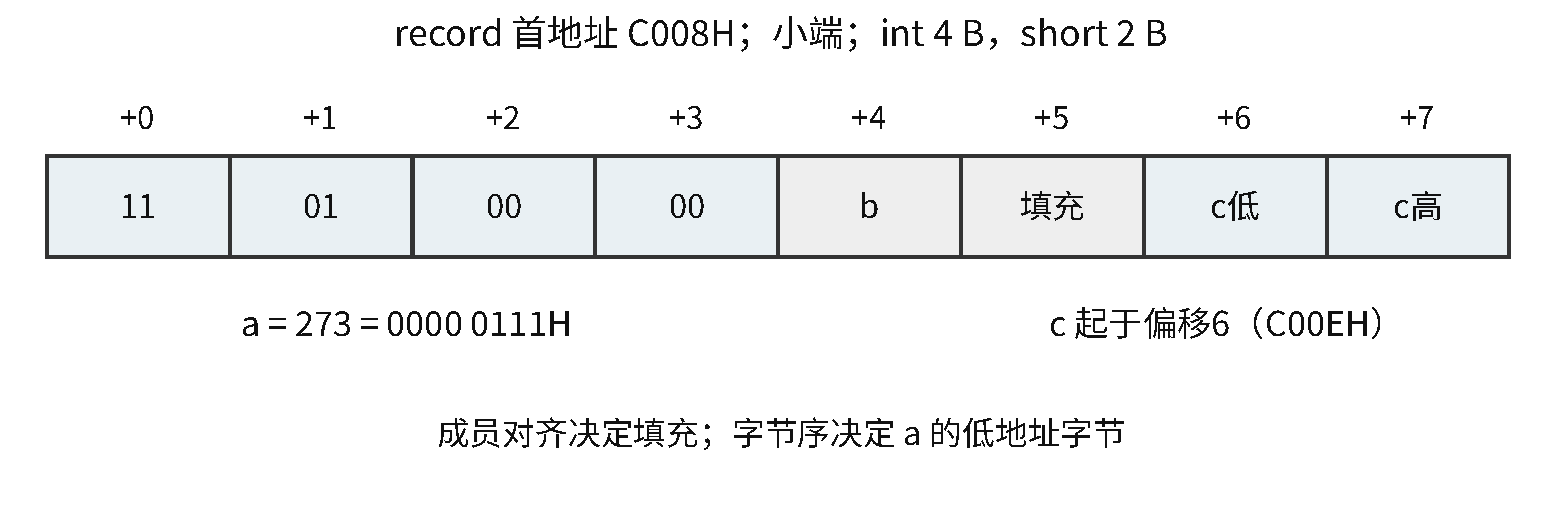
\includegraphics[width=\linewidth,height=125mm,keepaspectratio]{figures/CO_F05_struct_layout.pdf}
\captionof{figure}{结构体成员、填充与低地址字节分别标明}
\end{minipage}\par\medskip

二维数组按行优先存放时，\texttt{a[\allowbreak{}i]\allowbreak{}[\allowbreak{}j]\allowbreak{}} 的元素偏移为 \(i\times\text{列数}+j\)，字节偏移还要乘元素字节数。对于取负值的 short，先写出完整的16位补码，再按字节序拆开。例如\ensuremath{-}6为 \texttt{FFFAH}，小端低地址是FA、下一字节是FF，不是把真值“\ensuremath{-}6”拆成十进制字符。

\section{把位串、真值和条件分开核算}\label{CO02-method}

\begin{methodbox}[表示与运算题的统一路径]

先写位宽与编码，再求数学真值或完整精确结果；按题设完成截断、扩展或舍入，最后解释结果位串并检查标志。浮点解码先识别阶码的全0/全1，普通数公式不适用于特殊编码。涉及C代码时再核语言语义，不能把某种硬件结果提升为标准C保证。

\end{methodbox}

\subsection{补码为什么恰好多一个负数}\label{CO02-proof}

\begin{proof}[由位权得到范围]

\(n\)位补码的值是\(-b_{n-1}2^{n-1}+\sum_{i=0}^{n-2}b_i2^i\)。最小时只有符号位为1，值为\(-2^{n-1}\)；最大时符号位0而其余全1，值为\(\sum_{i=0}^{n-2}2^i=2^{n-1}-1\)。这既说明负数多一个，也说明最小负数的相反数无法放回同宽补码中。

\end{proof}

\subsection{精度与范围各问什么}\label{CO02-precision}

binary32在\([2^e,2^{e+1})\)内，相邻正规格化数相差\(2^{e-23}\)。原因是尾数字段每增加1，有效数增加\(2^{-23}\)，再乘指数倍率\(2^e\)。在\([2^{24},2^{25})\)间距为2，所以\(2^{24}+1\)无法精确保存；\(2^{25}\)本身却是精确的二进制幂。有限数是否溢出取决于指数边界，能否精确取决于有效位，两者不可互代。

最近偶数舍入先比较被舍弃部分与半个间隔：小于一半向较近值，大于一半向另一侧；恰好一半时选保留末位为0的候选。只写``四舍五入''会漏掉二进制等距点规则。

\subsection{对齐和容量的单位}\label{CO02-storage}

机器字长是CPU一次处理整数的基本宽度，存储字长是一个存储单元保存的位数，指令字长是某条指令的编码位数；三者可以不同。按字节编址时，32位整数通常占4个连续地址；按32位字编址时，同一个字只占一个地址。先把地址单位写出来，再计算数组偏移、总容量和跨界访问次数。

自然对齐要求对象起点满足某个倍数，但具体倍数来自题设或ABI。结构体末尾填充使数组中下一对象也满足对齐；删除末尾填充可能让第一个对象内部正确而第二个对象起点出错。字节序则只回答多字节值的高低有效字节如何落到地址，不能决定填充量。

\section{数字逻辑：从真值表到运算部件}\label{CO02-digital-logic}

逻辑运算把0、1解释为假、真。与运算只有输入全为1才输出1；或运算只要有输入为1就输出1；非运算反转一个输入；异或在两个输入不同时输出1，同或在两个输入相同时输出1。逻辑式中的``+''表示或，``乘积''表示与，不能直接当作整数加乘。

\begin{wideblock}\par\medskip\noindent\begin{minipage}{\linewidth}\fontsize{9.3}{12}\selectfont\begin{tabularx}{\linewidth}{@{}YYYY@{}}
\toprule\noalign{}
\(A,B\) & 与 \(AB\) & 或 \(A+B\) & 异或 \(A\oplus B\) \\
\midrule\noalign{}


0,0 & 0 & 0 & 0 \\
0,1 & 0 & 1 & 1 \\
1,0 & 0 & 1 & 1 \\
1,1 & 1 & 1 & 0 \\
\bottomrule\end{tabularx}
\end{minipage}\par\medskip\end{wideblock}

非、与、或的通常优先级依次降低；括号和非号覆盖范围优先明确。德摩根律为\(\overline{A+B}=\bar A\bar B\)、\(\overline{AB}=\bar A+\bar B\)。异或满足交换律和结合律，多个位异或的结果为1，当且仅当其中1的个数为奇数；这既可生成一位二进制加法的本位和，也可构造奇偶校验。

\subsection{选择器和三态门怎样控制通路}\label{CO02-mux-tristate}

\(k\)选1多路选择器MUX有\(k\)组数据输入、一组输出和选择信号，至少需要\(\lceil\log_2k\rceil\)位选择编码。2选1且选择位为\(s\)时，输出可写为\(Y=\bar sD_0+sD_1\)。若数据总线有32位，应把它理解为32路对应位一起被选择。

三态门除0、1外，还有高阻态。使能时输出跟随输入；关闭时输出端呈高阻，对公共总线不施加有效驱动。高阻态不是数值0。一条内部总线可连接多个输出端，但同一时刻必须按控制约束选择驱动源；多个源同时输出相反电平会发生总线争用。

\par\medskip\noindent\begin{minipage}{\linewidth}
\centering
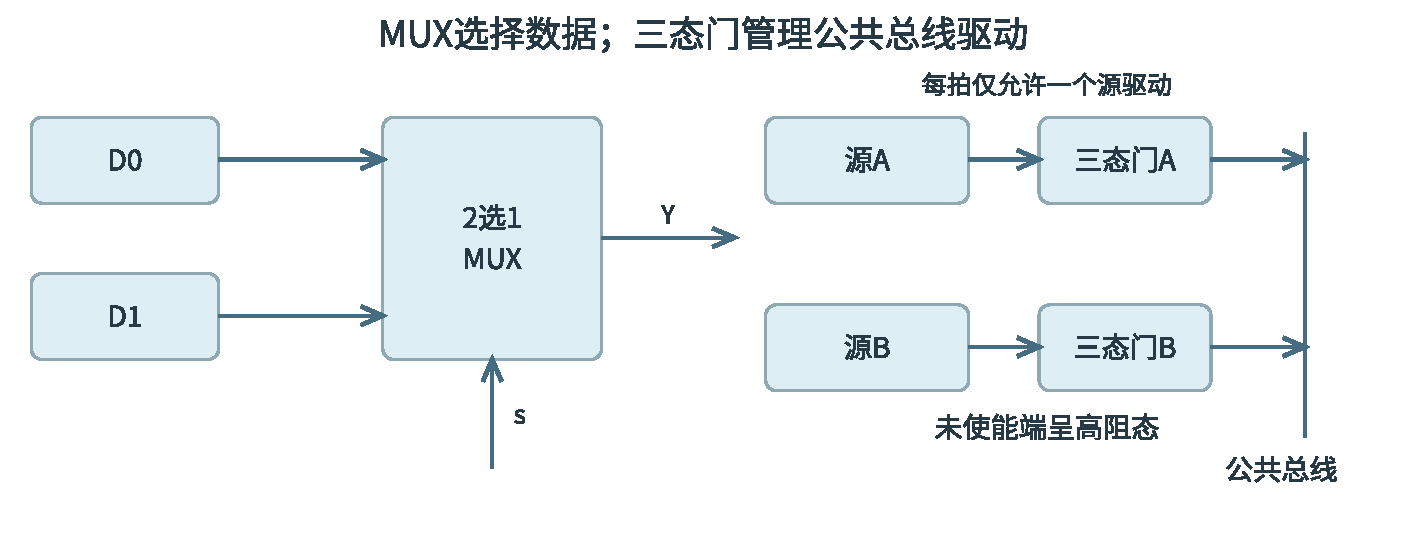
\includegraphics[width=\linewidth,height=125mm,keepaspectratio]{figures/CO02_mux_bus.pdf}
\captionof{figure}{选择器选择数据源，三态门决定输出端是否驱动公共线}
\end{minipage}\par\medskip

\subsection{全加器、进位产生与ALU选择}\label{CO02-adder-complete}

一位全加器输入\(A_i,B_i,C_{i-1}\)，输出本位和与进位：

\[S_i=A_i\oplus B_i\oplus C_{i-1},\qquad C_i=A_iB_i+(A_i\oplus B_i)C_{i-1}.\]

令\(G_i=A_iB_i\)为进位产生信号，\(P_i=A_i\oplus B_i\)为进位传播信号，则\(C_i=G_i+P_iC_{i-1}\)。继续代入可以写出\(C_2=G_2+P_2G_1+P_2P_1C_0\)。串行进位加法器逐级等待前一级进位；先行进位电路通过组合逻辑提前形成进位，以增加电路复杂度换取速度。

``并行加法器''可指多个输入位同时送入，并不保证进位也同时生成。ALU则在加法器和逻辑电路基础上，由操作控制位选择加、减、与、或、移位等功能；数据位宽与操作选择编码位宽是不同的量。

\section{乘法：按寄存器状态逐轮核算}\label{CO02-multiply-process}

\subsection{\texorpdfstring{无符号乘法：\(1101\times1011\)}{无符号乘法：1101\textbackslash times1011}}\label{CO02-unsigned-trace}

设\(n=4\)，被乘数寄存器\(X=1101\)，初始部分积\(P=0000\)、乘数\(Y=1011\)、进位\(C=0\)。每轮先根据\(Y\)最低位决定是否把\(X\)加到\(P\)，保留最高进位，再把\((C,P,Y)\)整体逻辑右移，重复4轮。

\par\medskip\noindent\begin{minipage}{\linewidth}\fontsize{9.3}{12}\selectfont\begin{tabularx}{\linewidth}{@{}YYY@{}}
\toprule\noalign{}
轮次 & \(Y\)最低位与加法结果 \(C,P\) & 整体右移后的 \(P,Y\) \\
\midrule\noalign{}


初始 & --- & 0000,1011 \\
1 & 1；0,1101 & 0110,1101 \\
2 & 1；1,0011 & 1001,1110 \\
3 & 0；0,1001 & 0100,1111 \\
4 & 1；1,0001 & 1000,1111 \\
\bottomrule\end{tabularx}
\end{minipage}\par\medskip

最终\((P,Y)=10001111_2=143=13\times11\)。完整乘积需要\(2n\)位；若结果字段仅保留低\(n\)位，则高\(n\)位非零表示无符号乘积不能由\(n\)位完整表示。课件中的硬件标志行为应与具体指令定义对应；C语言无符号类型运算按模\(2^n\)处理，而有符号溢出的语言语义另行规定。

\subsection{\texorpdfstring{Booth补码一位乘法：\(-3\times6\)}{Booth补码一位乘法：-3\textbackslash times6}}\label{CO02-booth-trace}

补码乘法让符号位参加运算。令\(X=1101\)表示\(-3\)，初始\(P=0000\)、\(Y=0110\)、辅助位\(q_{-1}=0\)。观察\((Y_0,q_{-1})\)：00、11执行\(+0\)，01执行\(+X\)，10执行\(-X\)。随后把\((P,Y,q_{-1})\)整体算术右移，保留最左符号位。

\par\medskip\noindent\begin{minipage}{\linewidth}\fontsize{9.3}{12}\selectfont\begin{tabularx}{\linewidth}{@{}YYY@{}}
\toprule\noalign{}
轮次 & 观察位与操作 & 算术右移后的 \(P,Y,q_{-1}\) \\
\midrule\noalign{}


初始 & --- & 0000,0110,0 \\
1 & 00，\(+0\) & 0000,0011,0 \\
2 & 10，\(-X\) & 0001,1001,1 \\
3 & 11，\(+0\) & 0000,1100,1 \\
4 & 01，\(+X\) & 1110,1110,0 \\
\bottomrule\end{tabularx}
\end{minipage}\par\medskip

乘积为\(11101110_2=-18\)。若只保留4位，则低4位1110表示\(-2\)，与真实乘积不同。对\(2n\)位补码乘积保留低\(n\)位，未溢出的条件是高\(n\)位均为低\(n\)位符号位的扩展，即最高\(n+1\)位全部相同。处理最小负数等边界时，需要足够的内部符号扩展，不能在过窄的临时寄存器中直接对最小负数求正值。

\subsection{硬件实现的三种组织}\label{CO02-multiply-hardware}

逐位乘法用同一加法器多次完成加法、移位，硬件少而周期多；阵列乘法器用更多组合电路并行形成部分积并累加，延迟取决于电路路径；流水线乘法器在组合逻辑中插入阶段寄存器，允许多组乘法交叠。流水线主要提高持续输入时的吞吐率，单次乘法仍要经历完整延迟。

\section{除法：先明确被除数、商和余数的位宽}\label{CO02-division-complete}

无符号双精度除法通常以\((R,Q)\)保存\(2n\)位被除数，除数寄存器保存\(n\)位除数，结束后\(Q\)保存商、\(R\)保存余数。单精度被除数先零扩展，带符号被除数则按约定作符号扩展。除数为0属于除法异常；商还必须落在目标字段的表示范围。

恢复余数法可理解为：移入下一被除数位，试减除数；若结果非负，上商1；若为负，加回除数恢复余数，上商0。不恢复余数法则利用当前余数符号决定下一轮加或减，减少``立即恢复''动作，但最终须按算法规则校正余数。

以\(1111_2\div0010_2\)，即\(15\div2\)为例，下面用逐位长除法呈现同一数学过程：

\par\medskip\noindent\begin{minipage}{\linewidth}\fontsize{9.3}{12}\selectfont\begin{tabularx}{\linewidth}{@{}YYY@{}}
\toprule\noalign{}
处理的被除数位 & 移入后的中间值 & 本位商、余数 \\
\midrule\noalign{}


第1位1 & 1 & 0，1 \\
第2位1 & \(2\times1+1=3\) & 1，1 \\
第3位1 & 3 & 1，1 \\
第4位1 & 3 & 1，1 \\
\bottomrule\end{tabularx}
\end{minipage}\par\medskip

得到商0111、余数0001，满足\(15=7\times2+1\)且\(0\le1<2\)。表中的长除法是数学核算模型，和硬件\((R,Q)\)整体移位时的寄存器切分应分别标明。

\subsection{双精度除法的商溢出与寄存器轨迹}\label{CO02-division-registers}

无符号\(2n\)位被除数先分装到\(R,Q\)，各\(n\)位，\(Y\)保存\(n\)位除数。\(Y>0\)时，若初始高半部\(R\ge Y\)，则商至少为\(2^n\)，不能装入\(n\)位\(Q\)；因此正式迭代前可先作商溢出检查。课件中的\(255/15=17\)超出4位商范围，而\(200/15=13\)余5可以表示。单精度无符号被除数先零扩展，高半部为0；除数非零时，商不会超出同宽无符号范围。

对\(15/2\)，初态为\(R=0000,Q=1111,Y=0010\)。每轮将\(RQ\)整体左移，使下一被除数位进入\(R\)，再试算\(R-Y\)：非负时保留差并把\(Q\)最低位置1；负时恢复原\(R\)并置0。循环4轮后，\(R\)为余数、\(Q\)为商。

\par\medskip\noindent\begin{minipage}{\linewidth}
\centering
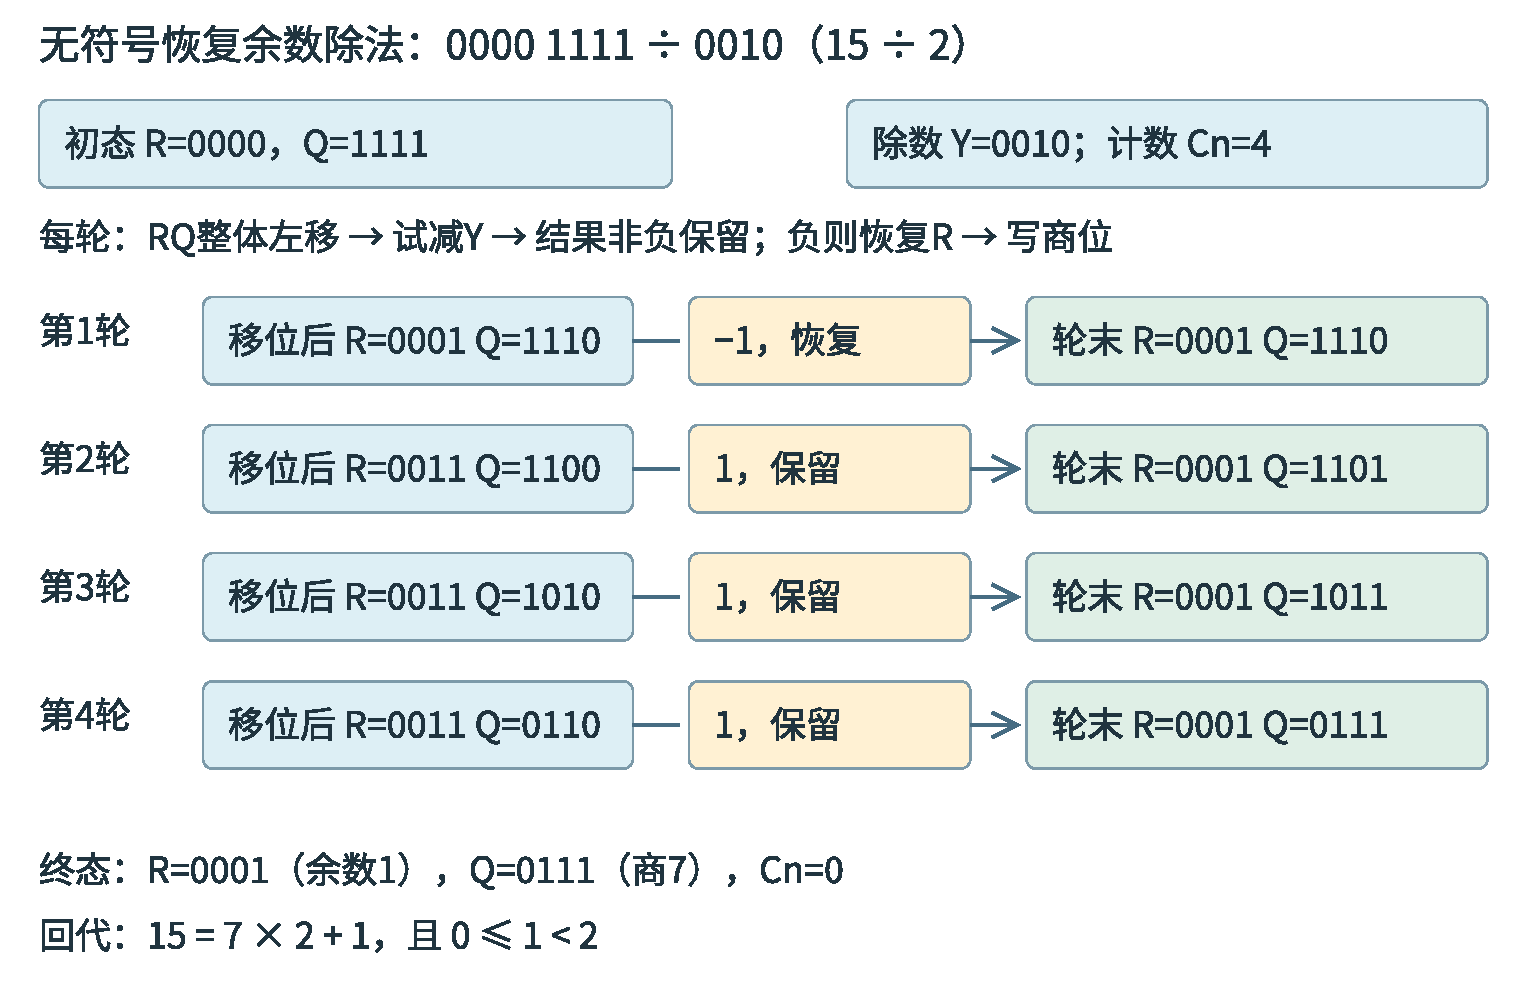
\includegraphics[width=\linewidth,height=125mm,keepaspectratio]{figures/CO02_restoring_division.pdf}
\captionof{figure}{王道课件15除以2的四轮寄存器状态，包含试减、恢复与商位写入}\label{co02-fig-division}
\end{minipage}\par\medskip

``试减为负''是临时结果，并不表示被除数变为带符号负数。电路须保存用于试算符号或借位判断的状态；把负的试算低位直接当作最终无符号余数，会破坏\(0\le R<Y\)。

\subsection{补码除法中的符号扩展和商修正}\label{CO02-signed-division-trace}

王道课件以4位补码\(-7/3\)说明有符号除法。被除数1001先符号扩展为8位，初态\(R=1111,Q=1001\)；除数\(Y=0011\)。下面列出这一实例的状态，\(R\)栏按4位补码解读。被除数与正除数异号，试算为\(R+Y\)，本例试算结果若改变余数原来的负号就恢复，否则保留并生成商的绝对值位。

\begin{wideblock}\par\medskip\noindent\begin{minipage}{\linewidth}\fontsize{9.3}{12}\selectfont\begin{tabularx}{\linewidth}{@{}YYYY@{}}
\toprule\noalign{}
轮次 & 移位后的R、Q & 试加后的R & 轮末R、Q \\
\midrule\noalign{}


1 & 1111、0010 & 0010，符号改变 & 恢复为1111、0010 \\
2 & 1110、0100 & 0001，符号改变 & 恢复为1110、0100 \\
3 & 1100、1000 & 1111，保留 & 1111、1001 \\
4 & 1111、0010 & 0010，符号改变 & 恢复为1111、0010 \\
\bottomrule\end{tabularx}
\end{minipage}\par\medskip\end{wideblock}

四轮后\(Q=0010\)是商的绝对值2。因原操作数异号，再对\(Q\)取补得到1110，即商\(-2\)；\(R=1111\)即余数\(-1\)，满足\(-7=(-2)\times3+(-1)\)。课件的另外两例为\(6/3=2\)余0，以及\(3/(-7)=0\)余3。表中没有出现试算恰为0的情形；一般电路还需单独正确处理整除，不能把``结果符号位变0''机械地判为试算失败。

也可先在足够宽的内部表示中求两数绝对值，按无符号规则求商余数，最后恢复商符号和余数符号；这是一种便于核算的等价模型。最小负数的绝对值需要保护位，不能直接在原来的\(n\)位补码寄存器中取正值。单精度补码除法还须预先排除除数0及最小负数除以\(-1\)两类异常。

带符号整数除法中，商符号由两操作数符号异或决定；按C语言向0截断的约定，非零余数与被除数同号，始终满足\(X=QY+R\)。例如\(-15/2=-7\)、余数\(-1\)；\(15/(-2)=-7\)、余数1。对\(n\)位补码，最小负数除以\(-1\)的商超出可表示范围，应单独判断。

\section{浮点数舍入的临界情形}\label{CO02-rounding-complete}

IEEE 754单精度规格化数含24位有效二进制精度。在\([2^{24},2^{25})\)范围内，相邻可表示数的间距为2；因此\(2^{24}+1\)恰好处于两个可表示数的中点。

最近偶数舍入的步骤是：先比较被舍部分与半个最低有效位；小于半单位截断，大于半单位进1；恰好半单位时，选择保留部分末位为0的结果。保留保护位、舍入位、粘滞位，可判断被舍部分的大小；粘滞位是更低所有被舍位的或。

\par\medskip\noindent\begin{minipage}{\linewidth}\fontsize{9.3}{12}\selectfont\begin{tabularx}{\linewidth}{@{}YYY@{}}
\toprule\noalign{}
加法 & 精确结果相对相邻浮点数的位置 & 单精度最近偶数结果 \\
\midrule\noalign{}


\(2^{24}+0.5\) & 距\(2^{24}\)更近 & 16777216 \\
\(2^{24}+1\) & 正好居中，低端末位偶 & 16777216 \\
\(2^{24}+1.5\) & 距\(2^{24}+2\)更近 & 16777218 \\
\((2^{24}+2)+1\) & 正好居中，高端末位偶 & 16777220 \\
\bottomrule\end{tabularx}
\end{minipage}\par\medskip

对阶导致移位不等于立刻丢弃全部低位；舍入可能再次产生尾数进位，需要右规并使指数增加。判断上溢应在规格化、舍入后检查指数；接近0的结果还要根据表示格式区分次正规数和下溢处理。

\subsection{计算与辨析自查}\label{CO02-extra-check}

\begin{enumerate}
\def\labelenumi{\arabic{enumi}.}
\tightlist
\item
  高阻态为什么不能当成数据0？2. \(n\)位补码乘积保留低\(n\)位时怎样判断溢出？3. \(-15=Q\times2+R\)按向0截断时\(Q,R\)分别是多少？4. 单精度数16777218加1为什么成为16777220？
\end{enumerate}

\textbf{答案。} 1. 高阻表示输出端不主动驱动总线，而0是主动输出低电平。2. 检查完整\(2n\)位结果是否为低\(n\)位的符号扩展。3. \(Q=-7,R=-1\)。4. 精确结果居中，最近偶数舍入选择有效尾数末位为0的高端数。

\section{主动回忆自测}\label{CO02-recall}

\subsection{配套自测}\label{CO02-27}

\begin{enumerate}
\def\labelenumi{\arabic{enumi}.}
\tightlist
\item
  原创补充：8位机器计算 \texttt{7FH+\allowbreak{}01H}，按本章标志约定求低8位结果、CF、OF、SF、ZF。
\item
  原创补充：binary32位串 \texttt{0000 0001H} 与 \texttt{0080 0000H} 各表示什么正数？两者是否都具有隐含前导1？
\item
  【配套例题】 已知32位 int 变量 i=12345，float 变量 \(f=1.2345\times2^3\)。下列结果为假的是：A. \texttt{i=\allowbreak{}=\allowbreak{}(\allowbreak{}int)\allowbreak{}(\allowbreak{}double)\allowbreak{}i}；B. \texttt{f=\allowbreak{}=\allowbreak{}(\allowbreak{}float)\allowbreak{}(\allowbreak{}double)\allowbreak{}f}；C. \texttt{i=\allowbreak{}=\allowbreak{}(\allowbreak{}int)\allowbreak{}(\allowbreak{}float)\allowbreak{}i}；D. \texttt{f=\allowbreak{}=\allowbreak{}(\allowbreak{}float)\allowbreak{}(\allowbreak{}int)\allowbreak{}f}。
\end{enumerate}

\textbf{答案。} 1. 结果 \texttt{80H}，CF=0、OF=1、SF=1、ZF=0；127+1越出补码范围，但未越出8位无符号范围。2. 分别为 \(2^{-149}\) 与 \(2^{-126}\)，前者非规格化、隐含0，后者规格化、隐含1。3. D。12345能被 binary32精确表示；float到double再回来也保留原float值，但 f 截断为整数会丢小数部分。

\subsection{遮住答案复述知识关系}\label{CO02-recall-new}

\begin{recallcard}[主动回忆·自拟]

\begin{enumerate}
\def\labelenumi{\arabic{enumi}.}
\setcounter{enumi}{3}
\tightlist
\item
  配套结构体案例：某32位计算机按字节编址、小端、int为4B，按自然边界对齐。结构为 \texttt{struct record \{ int id;\allowbreak{} char name[\allowbreak{}10]\allowbreak{};\allowbreak{} int salary;\allowbreak{} \} employee[\allowbreak{}200]\allowbreak{};\allowbreak{}}，数组首址A0B0H。若employee{[}1{]}.id为12345678H，其中56H的地址是多少？
\item
  自拟：8位补码最小负数取反加1得到自身，为什么不能据此说数学相反数等于自身？
\item
  自拟：解释8位补码\ensuremath{-}3算术右移1位和C整数\ensuremath{-}3/2为何可能不同。
\item
  自拟：binary32在\([2^{25},2^{26})\)的相邻间隔是多少？\(2^{25}+1\)按最近偶数舍入到哪里？
\item
  自拟：列出恢复余数和不恢复余数法都必须满足的最终商余数关系。
\item
  自拟：12345678H采用大端和小端时，最低地址分别保存哪一字节？字节中的位需要反转吗？
\end{enumerate}

\end{recallcard}

\subsection{参考答案}\label{CO02-answers}

\begin{enumerate}
\def\labelenumi{\arabic{enumi}.}
\setcounter{enumi}{3}
\tightlist
\item
  A0C5H。结构大小20B，第二元素首址A0C4H，小端56H位于其后1B。
\item
  同宽运算按模256保存位串；+128不在8位补码范围，不能把位串绕回当作数学等式。
\item
  算术右移复制符号位，\ensuremath{-}3变\ensuremath{-}2，相当于向负无穷取整；C整数除法向零截断得\ensuremath{-}1。还须核语言版本对负数右移的规定。
\item
  间隔4，\(2^{25}+1\)离\(2^{25}\)更近，舍入到\(2^{25}\)。
\item
  无符号被除数\(N=QD+R\)，\(D>0\)时\(0\le R<D\)；不恢复法可能需最终负余数校正。有符号还需给定商、余数符号及舍入约定。
\item
  大端12H、小端78H；不反转字节内部位。
\end{enumerate}
